\section{Introduction}

For this thesis a Java library called \verb|gp-modifiable-ast| was implemented. 
\verb|gp| stands for general purpose, meaning that it can provide the API for different grammars, for example for different programming languages.

\subsection{Motivation}

The motivation for this work came from a practical problem. 
While developing a large enterprise web application, there was a need to change the translation system.
A translation system is receiving a token as a string and returns a predefined translation depending on the target language.
This caused some issues, as the new translation system had a different call syntax as the old one.
This refactoring required looking into external data stored in a database for each different call the translation function.
Because of the dependency of external data, the automatic tools provided by the IDE have not been sufficient to refactor these calls.

On the other hand, this would have been a very time consuming task to perform manually, as over tenthousand calls to this function existed.

To resolve this issue, a specific JavaScript parser like Esprima \cite{esprima} was used. 
Esprima can parse JavaScript, provide an AST, allows modifications on the AST and conversion back to source code.
With this library it was possible to perform the refactoring with the necessary customization options and accuracy.

However, tools like Esprima mostly exist for well known programming languages, and each tool provides a different API.

While there are parser generators like SableCC \cite{sablecc}, which can generate parsers from a definition file, they are intended to be used for a different
purpose.
Common parser generators are implemented to provide a part of a compiler frontend, but they do not need to maintain whitespaces,
comments and be able to generate the original source code from the ast.

The goal of this work is to provide a library called \verb|gp-modifiable-ast| to minimize the effort needed to be able to perform manipulations directly on the AST and
beeing able to transform the AST back into source code with the least amount of changes needed.

The following example should illustrate that rewritable abstract syntax trees can be used for refactorings, which require some knowledge about the program structure.
The change that should be performed on the following source code is renaming all variables to enforce a camel case naming scheme on variables, while keeping
pascal case on function names. While this can be done with IDE tools, it would require manual effort every time.

Implementing a custom solution can enforce this naming scheme automatically.

\begin{lstlisting}[language=Java, caption=Example of untransformed code]
void should_be_snake_case(int should_be_camel_case) {
    int second_variable = should_be_camel_case;
}
\end{lstlisting}

The resulting AST from this code may look like this
\begin{figure}[H]
    \centering
    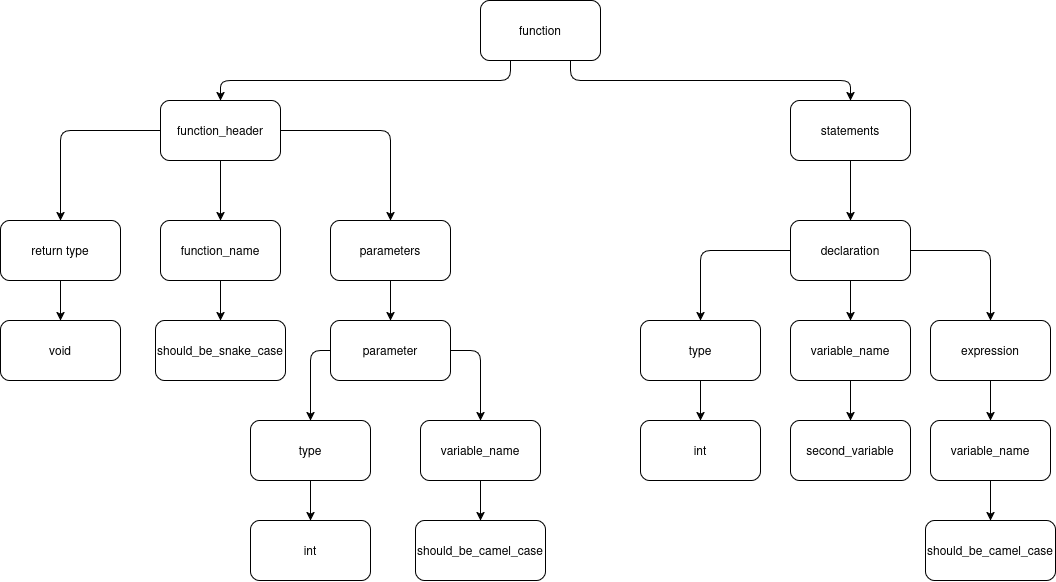
\includegraphics[scale=0.40]{fig/ast_example.png}
    \caption{AST example}
\end{figure}

This AST contains alot of informations about the program structure and allows to differentiate between variable and function names
\footnote{
    Depending on the grammar and language, this differentiation may not always be possible on the generated AST. 
    For example in JavaScript, functions can be passed as parameters into other functions: 
    \lstinline{function\_a(function\_b, variable\_a)}.
    The implemented LR(1) parser is not able to differentiate between the types of the parameters in this case.}. 

The following code should represent the general idea on how transformations on the AST could be implemented. 
The API of \verb|gp-modifiable-ast| is different from this example.

\begin{lstlisting}[language=Java, caption=Example of transformation]
    AST ast = parser.parse("example.java");
    List<ASTNode> nodes = ast.find("variable_name");
    renameToCamelCase(nodes);
    ast.transformBackToSourceCode();
\end{lstlisting}

This transformation would result in the following code.

\begin{lstlisting}[language=Java, caption=Example of transformation]
void should_be_snake_case(int shouldBeCamelCase) {
    int secondParam = firstParam;
}
\end{lstlisting}

This example should illustrate why rewritable abstract syntax trees can be a usefull tool for software development, as they allow a vast range of refactorings by containing
informations about the program structure.

\subsection{Related work}

The library implemented for this thesis (\verb|gp-modifiable-ast|) has similarities to common parser generators like SableCC \cite{sablecc}, ANTLR \cite{antlr}, GNU Bison \cite{gnu-bison} and others.

There are custom parsers like Esprima \cite{esprima}, which can generate a modifiable AST for JavaScript sources, but those are limited to one specific programming
language.

\verb|gp-modifiable-ast| is able to maintain the original formatting as much as possible and can be defined for any grammar that can be parsed by an LR(1) parser.

This work is based on the conference paper of Jeffrey L. Overbey and Ralph E. Johnson with the title "Generating Rewritable Abstract Syntax Trees" \cite{GeneratingRewritableAST}.
In this paper a possible grammar definition for rewritable abstract syntax trees is defined, which \verb|gp-modifiable-ast| implements partially. 
Some of the proposed definitions of \cite{GeneratingRewritableAST} have not been implemented, as those would not serve any purpose with the
structure of \verb|gp-modifiable-ast|. In chapter \ref{chap:ast_generation} it is discussed, which ones are implemented and which ones are not.